\documentclass[]{article}
\usepackage[T1]{fontenc}
\usepackage[utf8]{inputenc}
%% The early lwarp code will be inserted here.
\usepackage{iftex}
\usepackage{etoolbox}% for the fake-lwarp boolean
%% The early lwarp code will be inserted here.
\InputIfFileExists{ctikz-lwarp-early.tex}{%
        % this comment seems to be needed to avoid confusing lwarpmk
        % usepackage{lwarp}
    }{%
        %% define a couple of fake conditional for lwarp support
        \providebool{warpingHTML}
        \providebool{warpingprint}
        % Default: PDF build
        \boolfalse{warpingHTML}
        \booltrue{warpingprint}
}
\usepackage{imakeidx}
\ifbool{warpingprint}{%
    \makeindex[title=Index, intoc=true]
}{%
    \makeindex[title=Index, intoc=true, options={-s lwarp.ist}]
}
\indexprologue{Here you will find, in alphabetical order, all the components, keys, and styles defined by the package. Components have the page number in straight text, while keys and styles have \emph{italic} page numbers.}
\renewcommand*\seealso[2]{#2, \emph{\alsoname} #1}
\usepackage[siunitx, RPvoltages]{circuitikz}
\usepackage{ctikzmanutils}
\usepackage{imakeidx}
\ifbool{warpingprint}{%
    \makeindex[title=Index, intoc=true]
}{%
    \makeindex[title=Index, intoc=true, options={-s lwarp.ist}]
}
\indexprologue{Here you will find, in alphabetical order, all the components, keys, and styles defined by the package. Components have the page number in straight text, while keys and styles have \emph{italic} page numbers.}
\renewcommand*\seealso[2]{#2, \emph{\alsoname} #1}

\makeatletter
\makeatother

%% The late lwarp code will be inserted here.
%% {{{lwarp-late}}}
\ifbool{warpingprint}{}{\InputIfFileExists{ctikz-lwarp-late.tex}{}{}}
%
\usepackage[showframe]{geometry}
\begin{document}
\tableofcontents

\section{Dummy sec}\label{sec:dummy}
\subsection{Dummy subsec}\label{sec:dummy-dummy}
\subsubsection{Dummy subsubsec}\label{sec:dummy-dummy-dummy}

\begin{groupdesc}
    \circuitdesc*{bnc}{BNC connector}{}(left/135/0.6, right/45/0.6, center/-45/0.6, hot/0/0.6, zero/-135/0.6, shield/-90/0.4)
    \circuitdescbip[cuteopenswitch]{cute open switch}{Cute open switch\footnotemark}{cosw}(out/45/0.2)[out.s/-90/0.2]
    \footnotetext{Deferred footnote}
\end{groupdesc}

Here we\footnote{direct footnote} are...

\geolrcoord{bnc}

More text

\begin{lstlisting}
    A one
    B two
    C three
\end{lstlisting}





\begin{ctikzExample}[varwidth=true]
    \ctikzset{american}
    \tikz \draw (0,0) to[R=1<\ohm>] (4,0);

    \ctikzset{tallR/.style={
        resistors/scale=2, resistors/width=0.4}}
    \tikz \draw (0,0) to[R=1<\ohm>, tallR] (4,0);

    \ctikzset{european}
    \tikz \draw (0,0) to[R=1<\ohm>, tallR] (4,0);
\end{ctikzExample}

\begin{ctikzExample}[varwidth=true]
    \tikz \draw (0,0) to[R=1<\ohm>] (3,0);

    \ctikzset{resistors/width=2}
    \tikz \draw (0,0) to[R=1<\ohm>] (3,0);
\end{ctikzExample}

To change the height, you can use (locally) the class scale parameter and the width; you can even define a style that will work across the resistor styles:


\begin{ctikzExample}[]
    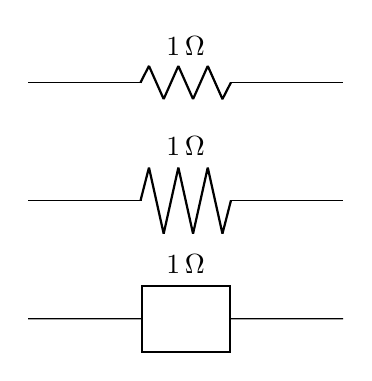
\begin{tikzpicture}[american]
        \draw (0,0) to[R=1<\ohm>] ++(4,0);
        \ctikzset{tallR/.style={
        resistors/scale=2, resistors/width=0.4}}
        \draw (0,-1.5) to[R=1<\ohm>, tallR] ++(4,0);

        \ctikzset{european}
        \draw (0,-3) to[R=1<\ohm>, tallR] ++(4,0);
    \end{tikzpicture}
\end{ctikzExample}

\par
\begin{ctikzExample}[varwidth=true, pos=t]
Plotted using \TikZ\ version \pgfversion{} and Circui\TikZ\ version \pgfcircversion{}.

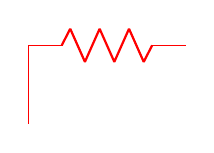
\begin{tikzpicture}
    \draw[color=red] (0,0) to[R] +(2,0) +(0,0) -- ++(0,-1);
\end{tikzpicture}
\qquad
\begin{tikzpicture}
    \draw[color=blue] (0,0) to[out=30, in=120] +(2,0) +(0,0) -- ++(0,-1);
\end{tikzpicture}
\qquad
\begin{tikzpicture}
    \draw[color=purple] (0,0) to[] +(2,0) +(0,0) -- ++(0,-1);
\end{tikzpicture}
\qquad
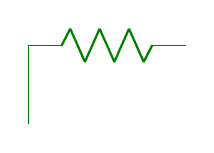
\begin{tikzpicture}
    \draw[color=green!50!black] (0,0)
        {[current point is local] to[R] +(2,0)} +(0,0) -- ++(0,-1);
\end{tikzpicture}
\end{ctikzExample}

Another example. First we define a \IndexKey{helper}
\begin{ctikzExample}[store=foo, only code]
\newcommand\foo[1]{bar#1bar}
\end{ctikzExample}
then we use it
\begin{ctikzExample}[restore=foo]
\foo{1}
\end{ctikzExample}

Yet another thingy thing
\begin{ctikzExample}[exec outside]
  \newcommand\foo{BAR}\foo
\end{ctikzExample}

\begin{ctikzExample}[only code, store=ChopperByTerminals]
\NewDocumentCommand{\ChopperByTerminals}{O{} O{0.2cm} m m m}{%
    % #1 -> options to the draw command
    % #2 -> half width
    % by default is drawn to the right (if vertical), to the left if #2 is negative
    % If horizontal, by default is above, below if #2 is negative
    % #3 -> terminal A on port 1
    % #4 -> terminal B on port 2
    % #5 -> name for the "anchors"
    \coordinate(#5-P1A) at (#3);
    \coordinate(#5-P1B) at (#4);
    % the center of the block is midway P1A to P1B, at distance #2 at 90 clockwise
    % degrees from the center of the line
    \coordinate(#5-C1) at ($(#5-P1A)!0.5!(#5-P1B)$);
    \coordinate(#5-C) at ($(#5-C1)!#2!90:(#5-P1B)$);
    \coordinate(#5-P2B) at ($(#5-P1A)!2!(#5-C)$);
    \coordinate(#5-P2A) at ($(#5-P1B)!2!(#5-C)$);
    \coordinate(#5-T1A) at ($(#5-P1B)!1.2!(#5-P1A)$);
    \coordinate(#5-T1B) at ($(#5-P1A)!1.2!(#5-P1B)$);
    \coordinate(#5-T2A) at ($(#5-P2B)!1.2!(#5-P2A)$);
    \coordinate(#5-T2B) at ($(#5-P2A)!1.2!(#5-P2B)$);
    \coordinate(#5-CKA) at ($(#5-T1A)!0.5!(#5-T2A)$);
    \coordinate(#5-CKB) at ($(#5-T1B)!0.5!(#5-T2B)$);
    \coordinate(#5-C2) at ($(#5-P2A)!0.5!(#5-P2B)$);
    \draw [draw, thick, fill=white, #1] (#5-T1A) rectangle (#5-T2B);
    \draw [draw, thick, line join=round, #1] (#5-P1A) -- (#5-P2B) --
        (#5-P1B) -- (#5-P2A) -- (#5-P1A);
}
\end{ctikzExample}

You can use this definition as follows, for example:

\begin{ctikzExample}[pos=b, restore=ChopperByTerminals, dollar]
\begin{tikzpicture}[]
    \node[op amp](A) at (0,0) {};
    \ChopperByTerminals[draw=red][-0.2cm]{A.-}{A.+}{chopper in}
    \draw [red, <-] (chopper in-CKA) -- ++(0,.5) node[above]{$f_c$};
    \ChopperByTerminals[draw=red]{[xshift=1.2cm]A.-}{[xshift=1.2cm]A.+}{chopper out}
    \draw [red, <-] (chopper out-CKA) -- ++(0,.5) node[above]{$f_c$};
    %Try another one
    \draw (4,1) node[npn](Q1){} (7,1) node[npn, xscale=-1](Q2){};
    \coordinate (Qcenter) at ($(Q1.E)!0.5!(Q2.E)$);
    \ChopperByTerminals[][-0.2cm]{Q1.E}{Q2.E}{cE}
    \draw [<-] (cE-CKA) -- ++(-0.5,0) node[left]{$f_c$};
    % pseudo-anchors
    \ChopperByTerminals[draw=blue][-1cm]{4,-1.25}{7,-1.25}{C}
    \foreach \a in {P1A, P1B, P2A, P2B, CKA, CKB, C, C1, C2}
        \node[circle, draw, inner sep=1pt, pin={[font=\tiny, fill=white]60:C-\a}]
            at (C-\a) {};
\end{tikzpicture}
\end{ctikzExample}

Let's see that with an example:

\begin{ctikzExample}[exec outside]
\ctikzsubcircuitdef{optovishay}{in 1, out 1, in 2, out 2, center}{%
    % reference anchor is -center
    coordinate(#1-center)
    (#1-center) +(-1.2,-1) rectangle +(1.2,1)
    (#1-center) ++(-1.2,0.8) coordinate (#1-in 1)
    (#1-center) ++(-1.2,-0.8) coordinate (#1-in 2)
    (#1-center) ++(1.2,0.8) coordinate (#1-out 1)
    (#1-center) ++(1.2,-0.8) coordinate (#1-out 2)
    (#1-center) ++(0,1) coordinate (#1-up)
    (#1-in 1) -- ++(0.5,0) coordinate(#1-tmp)
        to[leD*, diodes/scale=0.6, led arrows from cathode]
        (#1-tmp|- #1-in 2) -- (#1-in 2)
    (#1-out 1) -- ++(-0.5,0) coordinate(#1-tmp)
        to[pD*, diodes/scale=0.4, mirror]  ++(0,-0.5)
        edge[densely dashed] ++(0,-0.533) ++(0,-0.566)
        to[pD*, diodes/scale=0.4,mirror] (#1-tmp|- #1-out 2) -- (#1-out 2)
    % leave the position of the path at the center
    (#1-center)
}
\end{ctikzExample}

Our element is a symbol for an optocoupler; in this case is the symbol used for one cell of the double \href{https://www.vishay.com/docs/84639/vo1263aa.pdf}{Vishay vo1263 device}.

To use the subcircuit, an additional step is needed. Somewhere you have to \emph{activate} it. This is needed to calculate the relative positions of anchors using the current set of style parameters. The normal place is to activate it just before usage; to do that you use the command \verb|\ctikzsubcircuitactivate| with the name of the subcircuit. That will define a new command, \texttt{\textbackslash\emph{nameofthesubcircuit}} that you can use then in your paths.

So to check your subcircuit while defining it you can use this simple snippet:


\begin{ctikzExample}[only code]
\ctikzsubcircuitactivate{optovishay}
\end{ctikzExample}
% \ctikzsubcircuitactivate{optovishay}


\begin{ctikzExample}
\begin{tikzpicture}
% \ctikzsubcircuitactivate{optovishay}
    \draw (0,0) \optovishay{one}{};
    \node [above] at (one-up) {O1};
    \draw[color=blue] (one-out 1) -- ++(1,0)
        \optovishay{two}{in 1};
    \node [above] at (two-up) {O2};
\end{tikzpicture}
\end{ctikzExample}

\begin{ctikzExample}[only code]
\ctikzsubcircuitactivate{optovishay}
\end{ctikzExample}

\begin{ctikzExample}
\begin{tikzpicture}[scale=0.8, transform shape]
\ctikzsubcircuitactivate{optovishay}
    \draw (0,0) \optovishay{three}{};
    \draw (three-out 1) -- ++(0.5,0) coordinate(here);
    \begin{scope}[xscale=-1,rotate=-45,transform shape]
        \draw (here) \optovishay{four}{out 1};
    \end{scope}
    \draw[blue] (three-out 2) -| (four-out 2);
\end{tikzpicture}
\end{ctikzExample}


\subsection{An example with the \texttt{compatibility} option}
\label{ex:compatibility}

\IfFileExists{compatibility.pdf}{\fbox{\includegraphics{compatibility.pdf}}}{}%

\begin{lstlisting}
\documentclass{standalone}

\usepackage{tikz}
\usetikzlibrary{circuits.ee.IEC}
\usetikzlibrary{positioning}

\usepackage[compatibility]{circuitikzgit}
\ctikzset{bipoles/length=.9cm}

\begin{document}
 \begin{tikzpicture}[circuit ee IEC]
  \draw (0,0) to [resistor={name=R}] (0,2)
	to[diode={name=D}] (3,2);
  \draw (0,0) to[*R=$R_1$] (1.5,0) to[*Tnpn] (3,0)
    to[*D](3,2);
 \end{tikzpicture}
\end{document}
\end{lstlisting}



\printindex

\end{document}
